%%%%%%%% ICML 2022 EXAMPLE LATEX SUBMISSION FILE %%%%%%%%%%%%%%%%%

\documentclass[nohyperref]{article}

% Recommended, but optional, packages for figures and better typesetting:
\usepackage{microtype}
\usepackage{graphicx}
\usepackage{subfigure}
\usepackage{booktabs} % for professional tables
\usepackage{stfloats}
\usepackage{placeins}

% hyperref makes hyperlinks in the resulting PDF.
% If your build breaks (sometimes temporarily if a hyperlink spans a page)
% please comment out the following usepackage line and replace
% \usepackage{icml2023} with \usepackage[nohyperref]{icml2023} above.
\usepackage{hyperref}


% Attempt to make hyperref and algorithmic work together better:
\newcommand{\theHalgorithm}{\arabic{algorithm}}

% Use the following line for the initial blind version submitted for review:
\usepackage{icml2023}

% If accepted, instead use the following line for the camera-ready submission:
% \usepackage[accepted]{icml2023}

% For theorems and such
\usepackage{amsmath}
\usepackage{amssymb}
\usepackage{mathtools}
\usepackage{amsthm}

% if you use cleveref..
\usepackage[capitalize,noabbrev]{cleveref}

%%%%%%%%%%%%%%%%%%%%%%%%%%%%%%%%
% THEOREMS
%%%%%%%%%%%%%%%%%%%%%%%%%%%%%%%%
\theoremstyle{plain}
\newtheorem{theorem}{Theorem}[section]
\newtheorem{proposition}[theorem]{Proposition}
\newtheorem{lemma}[theorem]{Lemma}
\newtheorem{corollary}[theorem]{Corollary}
\theoremstyle{definition}
\newtheorem{definition}[theorem]{Definition}
\newtheorem{assumption}[theorem]{Assumption}
\theoremstyle{remark}
\newtheorem{remark}[theorem]{Remark}

% Todonotes is useful during development; simply uncomment the next line
%    and comment out the line below the next line to turn off comments
%\usepackage[disable,textsize=tiny]{todonotes}
\usepackage[textsize=tiny]{todonotes}


% The \icmltitle you define below is probably too long as a header.
% Therefore, a short form for the running title is supplied here:
\icmltitlerunning{Geodesic Integrated Gradients}

\begin{document}

\twocolumn[
\icmltitle{Using the Path of Least Resistance to Explain Deep Networks}

% It is OKAY to include author information, even for blind
% submissions: the style file will automatically remove it for you
% unless you've provided the [accepted] option to the icml2022
% package.

% List of affiliations: The first argument should be a (short)
% identifier you will use later to specify author affiliations
% Academic affiliations should list Department, University, City, Region, Country
% Industry affiliations should list Company, City, Region, Country

% You can specify symbols, otherwise they are numbered in order.
% Ideally, you should not use this facility. Affiliations will be numbered
% in order of appearance and this is the preferred way.
\icmlsetsymbol{equal}{*}

\begin{icmlauthorlist}
\icmlauthor{Joseph Enguehard}{comp}
\icmlauthor{Sina Salek}{comp}
\end{icmlauthorlist}

\icmlaffiliation{comp}{Babylon Health, 1 Knightsbridge Grn, London SW1X 7QA United Kingdom}

\icmlcorrespondingauthor{Joseph Enguehard}{joseph.enguehard@babylonhealth.com}

% You may provide any keywords that you
% find helpful for describing your paper; these are used to populate
% the "keywords" metadata in the PDF but will not be shown in the document
\icmlkeywords{Machine Learning, ICML}

\vskip 0.3in
]

% this must go after the closing bracket ] following \twocolumn[ ...

% This command actually creates the footnote in the first column
% listing the affiliations and the copyright notice.
% The command takes one argument, which is text to display at the start of the footnote.
% The \icmlEqualContribution command is standard text for equal contribution.
% Remove it (just {}) if you do not need this facility.

\printAffiliationsAndNotice{}  % leave blank if no need to mention equal contribution
% \printAffiliationsAndNotice{\icmlEqualContribution} % otherwise use the standard text.

\begin{abstract}
Integrated Gradients (IG), a widely used path-based attribution method, assigns importance scores to input features by integrating gradients of the models along a straight path from a baseline to the input. While effective in certain cases, we show that choosing straight paths can lead to flawed attributions. In this paper, we identify how these misattributions arise. As a solution, we propose a new approach that considers the input space as a Riemannian manifold and computes attributions by integrating gradients of the model along geodesics. We call our approach \emph{Geodesic Integrated Gradients}. To approximate geodesic paths, we introduce two methods: a \emph{k}-nearest neighbour-based approach for simpler models and a Stochastic Variational Inference-based method for more complex ones. Furthermore, in our experiments with both synthetic and real world data, we demonstrate that our approach outperforms existing explainability methods including the original IG.
\end{abstract}

\section{Introduction}
\label{sec:introduction}

The use of deep learning models has risen in many applications. With it, so too has the desire to understand why these models make certain predictions. These models are often referred to as ``opaque'', as it is difficult to discern the reasoning behind their predictions \citep{marcus2018deep}. Additionally, deep learning models can inadvertently learn and perpetuate biases found in their training data \citep{sap2019risk}. To create fair and trustworthy algorithms, it is essential to be able to explain a model's output \citep{das2020opportunities}. 

Some examples of the methods proposed to explain neural networks include Gradient SHAP \cite{lundberg2017unified}, Integrated Gradients  \citep{sundararajan2017axiomatic} and  \citep{kapishnikov2021guided}.

Significant effort has been dedicated to designing explanation methods that satisfy certain desirable axioms. This is due to the lack of ground truth for evaluating them. The axioms can ensure that the explanations are principled. One of the most successful axiomatic methods is Integrated Gradients (IG) \citep{sundararajan2017axiomatic}. Consider a function $f : R^n \to R$, representing the neural network and an input vector $\textbf{x} \in R^n$. Furthermore, consider a baseline input vector $\overline{\textbf{x}} \in R^n$ (typically chosen such that the network gives baseline a near zero score). IG explains the network by quantifying how much of the difference $f(\textbf{x}) - f(\overline{\textbf{x}})$ can be attributed to the $i$th dimension of $\textbf{x}$, $\textbf{x}_i$.

Integrated Gradient gives attribution $IG_i$ to the $i$th dimension of the input by solving the following path integral
\begin{equation}
IG_i(\textbf{x}) = (\textbf{x}_i - \overline{\textbf{x}}_i) \int_0^1 \frac{\partial f(\gamma(t))}{\partial \textbf{x}_i} dt, \label{eq:igi}
\end{equation}
where $\gamma(t) = \overline{\textbf{x}} + t(\textbf{x} - \overline{\textbf{x}})$ is a straight path from the baseline to input. The claim of the creators of IG is that Eq. \ref{eq:igi} tells us how the model got from predicting essentially nothing at $\overline{\textbf{x}}$ to giving the prediction at $\textbf{x}$. Considering gradients represent the rate of change of functions, the above expression should tell us how scaling each feature along the path affects the increase in the network score for the predicted class.

\begin{figure}[t!]
	\begin{center}
		\centerline{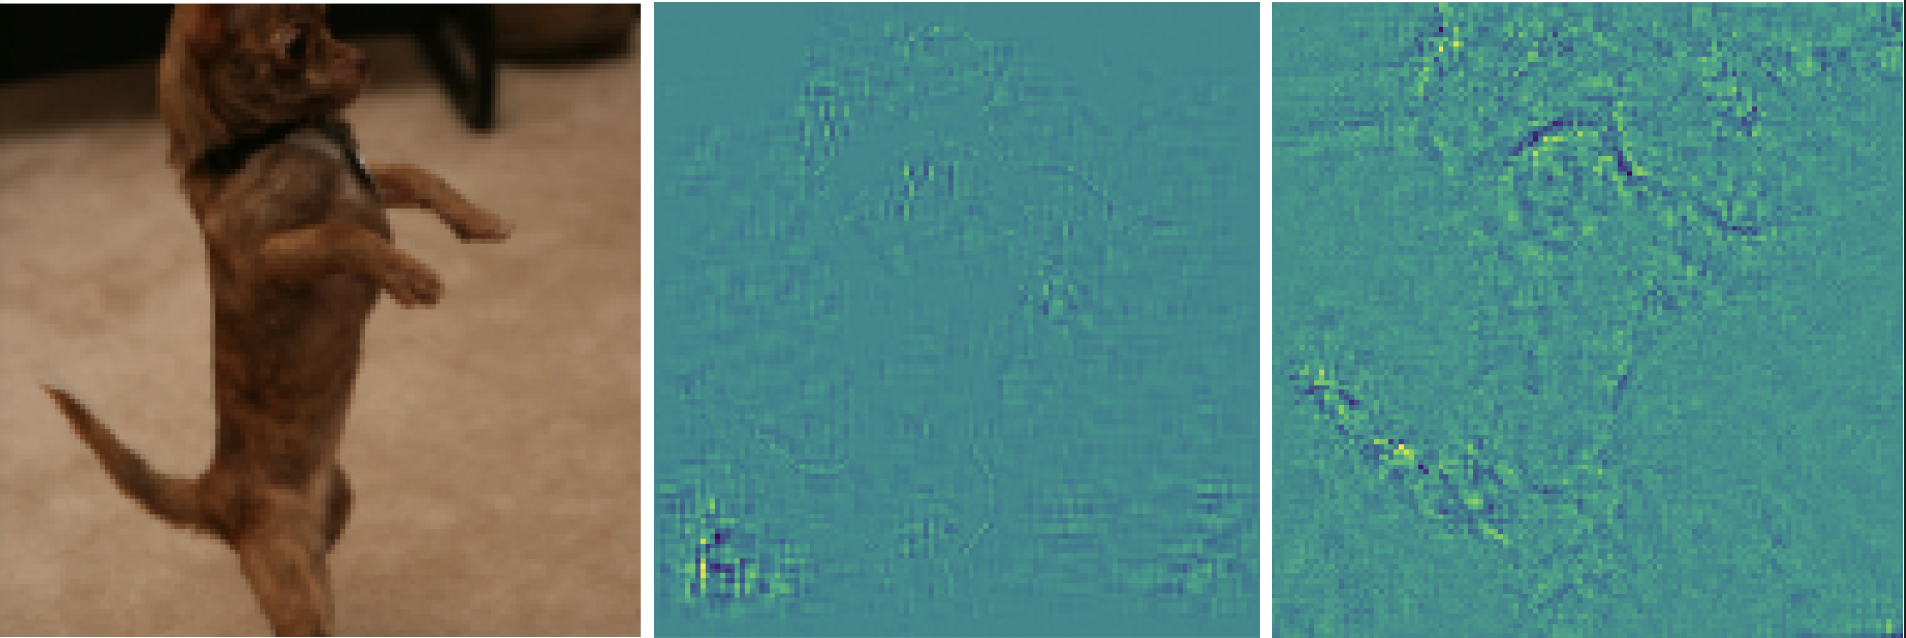
\includegraphics[width=0.95\columnwidth]{figures/voc_compare.png}}
		\caption{Comparison of attributions generated by Integrated Gradients (middle image) and Geodesic Integrated Gradients (right image). Integrated Gradients follow straight paths in Euclidean space, which can result in misleading attributions. In contrast, Geodesic Integrated Gradients integrate along geodesic paths on a Riemannian manifold defined by the model, correcting the misattributions due to poor alignment with the model's gradient landscape.}
		\label{fig:duck}
	\end{center}
	\vskip -0.3in
\end{figure}

In this paper, we demonstrate that defining attributions along straight paths in Euclidean space can lead to flawed explanations. We examine the consequences of these issues through examples in computer vision, as shown in Fig. \ref{fig:duck}, along with simpler, illustrative cases in Fig. \ref{fig:ig}. To address these challenges, we introduce \textbf{Geodesic Integrated Gradients} \footnote{The code for the attribution methods and reproducing the experiments is provided on \href{https://github.com/sina-salek/geodesic-ig}{https://github.com/sina-salek/geodesic-ig}}, a generalisation of IG that replaces straight paths with geodesic ones. These geodesics are defined on a Riemannian manifold, characterised by the model's input space and a metric induced by the model's gradients. This approach mitigates the identified pitfalls while retaining all the axioms of IG.

Before making the case for our Geodesic Integrated Gradient, let us first show an example of an artefact that can arise from choosing straight paths, generating explanations which do not reflect the true behaviour of a model. 

We highlight this issue on a half-moons classification task. We train a simple multi-layer perceptron (MLP) with 3 layers, ReLU activations and a cross-entropy loss to distinguish the upper moon from the lower one. The cross-entropy is split into a final log-softmax activation and a negative log-likelihood loss, so that we can explain probabilities.

We now compute Integrated Gradients, Eq. \ref{eq:igi}, for this model on the test data. Let us consider a baseline and input pair, such that the baseline is outside of either half-moon, for example at (-0.5, -0.5). This is a good choice of baseline, since network should assign near-zero score to it. Let us call the feature in the vertical axis the $1$st component of $x$. In Fig. \ref{fig:ig} we illustrate the attribution of this feature, $IG_1(\textbf{x})$, for each point using the colour map. One should expect to see all the points sufficiently above the decision boundary to receive equally high attributions. Intuitively, this is expected, because if a point is above the decision boundary, its $x_1$ component is an important factor in the classification. However, for a model that is very skillful at the classification task, since the point is significantly above the decision boundary, going slightly down should not make any difference. Because in such a model's score should not change significantly anywhere other than near the decision boundary. However, we can see in Fig. \ref{fig:ig} that some points on the upper moon receive much higher $x_1$-attribution than others. These are points such that a straight line from the baseline to them mostly falls on high gradient regions. This does not reflect the model's behaviour. A similar point could be made about the horizontal axis. This is in contrast with Fig. \ref{fig:ig}, where we show our method gives equally high attribution to all points sufficiently above the decision boundary, with different shades for the points closer to the boundary in $x_1$ direction. In Section \ref{subsec:half-moons} we present the details of how our method that achieves the results presented in this figure.

\begin{figure}[t!]
\vskip -0.1in
\begin{center}
\centerline{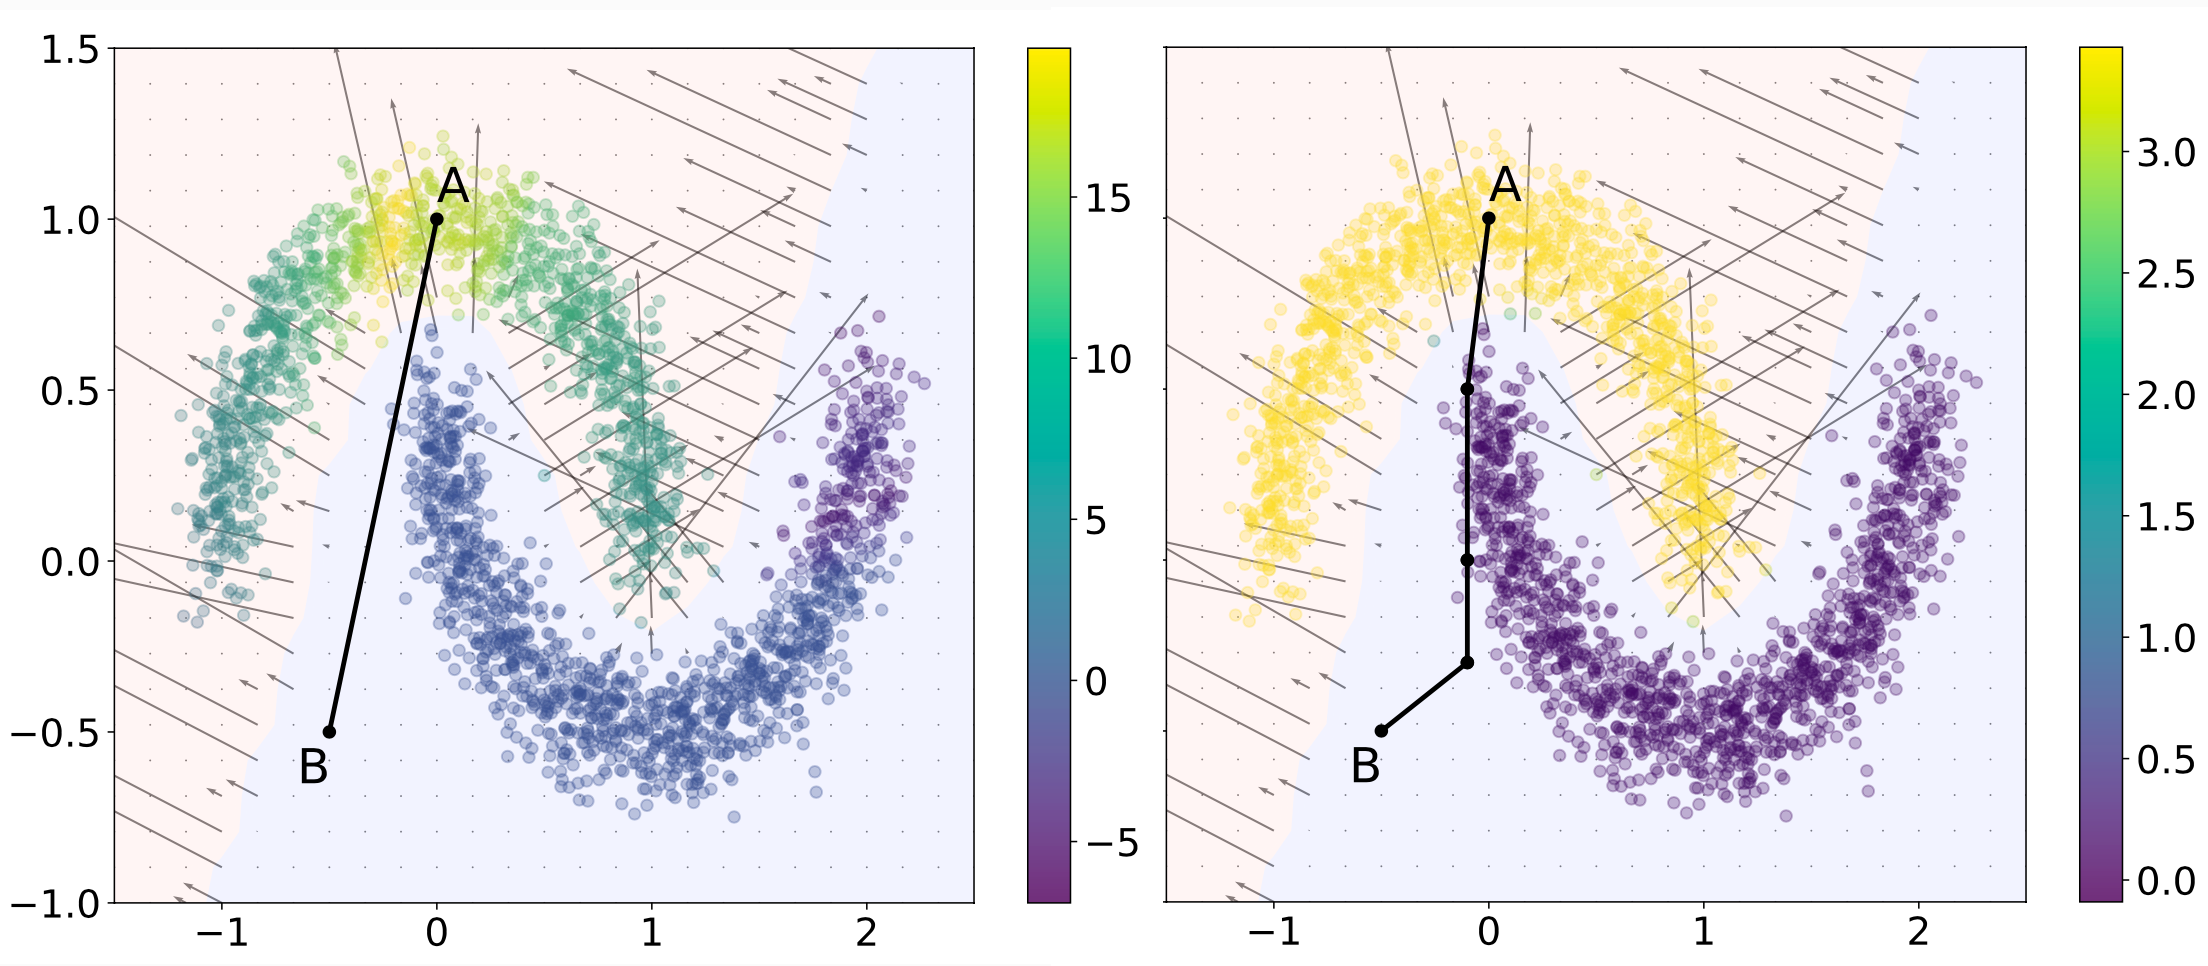
\includegraphics[width=\columnwidth]{figures/half_moons_y.png}}
\vskip -0.2in

\caption{\textbf{Integrated Gradients (IG) attributions (left) vs. Geodesic IG (right).} The colour map shows feature attributions on the vertical axis, with $(-0.5, -0.5)$ (point B) as the baseline. In IG, points near $A$ are over-attributed due to the straight path crossing high-gradient regions near the decision boundary (gray arrows). Geodesic IG avoids this issue by following geodesic paths, providing more accurate attributions.}
\label{fig:ig}
\end{center}
\vskip -0.2in
\end{figure}

\begin{figure}[!hbp]
	\vskip 0.2in
	\begin{center}
		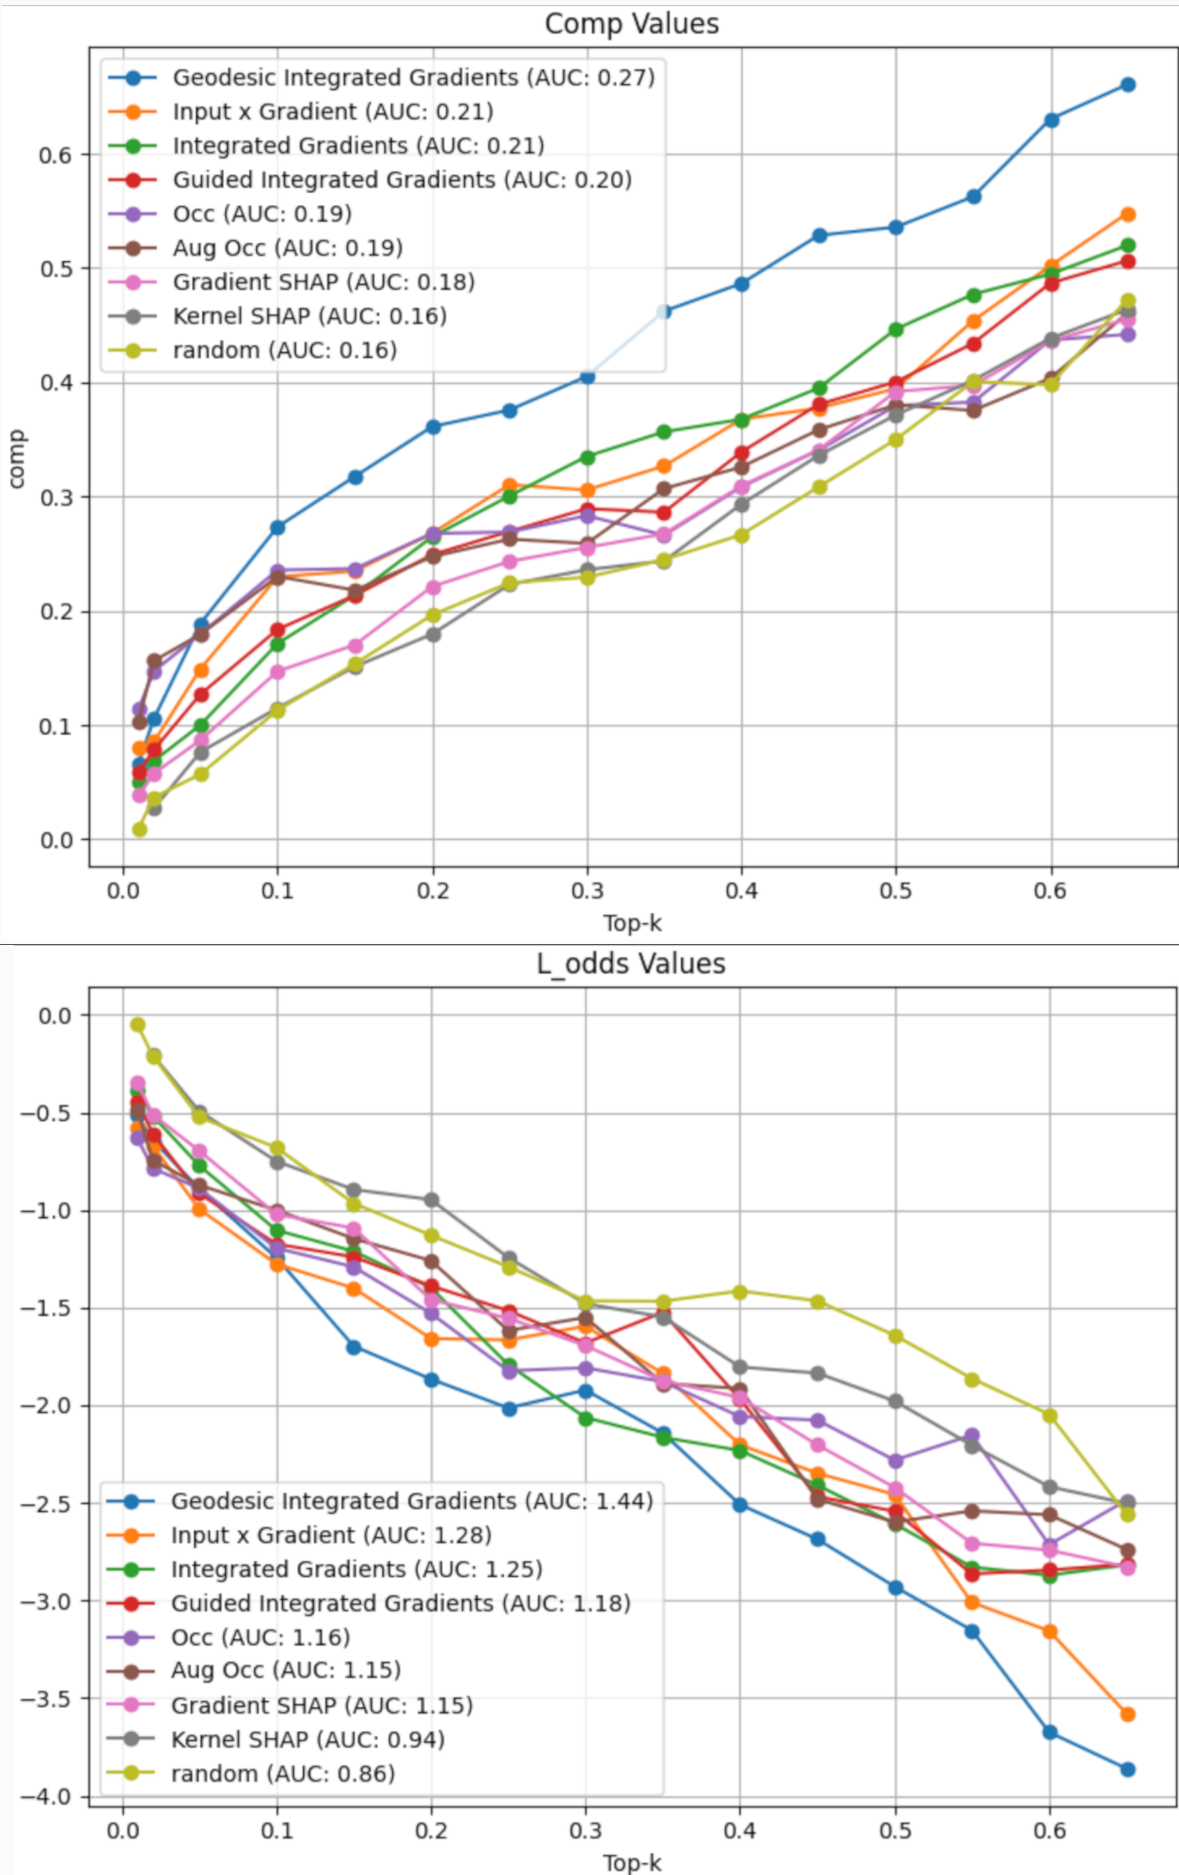
\includegraphics[width=0.85\columnwidth]{figures/voc_metrics_vertical.png}
		\caption{ \textbf{Metrics Comparison.} We use a ConNext model for classification of images from the VOC dataset. The horizontal axis represents the top $k\%$ (in absolute value) of features being selected. The top plot, \textit{Comprehensiveness}, shows the average change in the predicted class probability of compared to the original image (higher is better). The bottom plot displays the negative logarithmic probabilities of the predicted class relative to the original (lower is better). In both cases, the results are summarised using AUC, where higher values are better for both.}
		\label{fig:voc_metrics}
	\end{center}
	\vskip -0.2in
\end{figure}

Before giving the formal method in section \ref{sec:method}, let us discuss the intuition behind our Geodesic IG. We want the path in Eq. \ref{eq:igi} to be such that it avoids regions with high model gradient. This is because failing to do so would superficially increase the result of the integral, leading to the types of artefacts illustrated in Fig. \ref{fig:ig}. Therefore, we should try to find the path of least resistance, as this is the path that avoids steep gradients as much as possible. As we shall see in section \ref{sec:method}, the input space can be viewed as a Riemannian manifold with a metric derived from the model gradients. The path of least resistance between a chosen baseline and input, therefore, is the geodesic path between the two points.

In Section \ref{sec:method}, we present two methods for approximating the geodesic path between two points on a manifold. The first method, based on $k$-nearest neighbors ($k$NN), is designed for simpler manifolds, while the second method, utilising Stochastic Variational Inference, is suited for more complex manifolds. We further demonstrate that Geodesic IG adheres to all the axioms of Integrated Gradients.


In Section \ref{sec:experiments}, we demonstrate the effectiveness of the Geodesic IG method on the real-world Pascal VOC 2012 dataset \citep{pascal-voc-2012}. Our results outperform existing methods, as we evaluate using two metrics. We preview the results of this experiment in Fig. \ref{fig:voc_metrics}.

Section \ref{sec:related_work} reviews related work, including the comparison of Geodesic IG with other methods that attempt to overcome the shortcomings of Integrated Gradients.
\section{Method}
\label{sec:method}

In section \ref{sec:introduction}, we gave the intuition that using geodesic paths can correct the misattribuion in IG that arise from integrating along straight paths. Let us now formalise this idea.

\subsection{Geodesic distance formulation.} Let us define a neural network as a function $f: \mathbb{R}^n \to \mathbb{R}$, where $n$ is the dimension of the input space. Let us also define $\textbf{x}$ a point in this input space. We denote the Jacobian of $f$ at $\textbf{x}$ as $\textrm{J}_{\textbf{x}}$.

Using Taylor's theorem, for a vector $\boldsymbol{\delta}$ with an infinitesimal norm: $\forall \epsilon, ||\boldsymbol{\delta}|| \le \epsilon$, we have:

\begin{align}
\begin{split}
    ||f(\textbf{x} + \boldsymbol{\delta}) - f(\textbf{x})|| \approx ||\textrm{J}_{\textbf{x}}\boldsymbol{\delta}|| \approx \boldsymbol{\delta}^T \textrm{J}_{\textbf{x}}^T \textrm{J}_{\textbf{x}} \boldsymbol{\delta}
\end{split}
\label{eq:taylor}
\end{align}

Using equation \ref{eq:taylor}, we can now define a tangent space $\textrm{T}_\textbf{x}\textrm{M}$ of all $\boldsymbol{\delta}$, equipped with a local inner product $\textrm{G}_\textbf{x}$:

\begin{equation}
    <\boldsymbol{\delta}, \boldsymbol{\delta'}>_\textbf{x} = \boldsymbol{\delta}^T \textrm{G}_\textbf{x} \boldsymbol{\delta'}
    = \boldsymbol{\delta}^T \textrm{J}_{\textbf{x}}^T \textrm{J}_{\textbf{x}}\boldsymbol{\delta'}
\label{eq:inner_product}
\end{equation}

As a result, we can view the input space as a Riemannian manifold $(\mathbb{R}^n, \textrm{G})$, where the Riemannian metric $\textrm{G}$ is defined above. On this manifold, the length of a curve $\gamma(t): [0, 1] \to \mathbb{R}^n$ is defined as:

\begin{align}
\begin{split}
    \textrm{L}(\gamma) &= \int_0^1 \sqrt{<\dot \gamma(t), \dot \gamma(t)>_{\gamma(t)}}dt \\
    &= \int_0^1 ||\partial_t f(\gamma(t)) \times \dot\gamma(t)|| \, dt,
\end{split}
\label{eq:length}
\end{align}
where $\dot\gamma(t)$ is the derivative of $\gamma(t)$ with respect to $t$.
The \textbf{geodesic distance}, denoted $\textrm{L}^*$, between $\textbf{a}$ and $\textbf{b}$ is then defined as the minimum length among curves $\gamma$ such that $\gamma(0) = \textbf{a}$ and $\gamma(1) = \textbf{b}$. We also call \textbf{geodesic path} the curve $\gamma^*$ which minimises the length L. This path can be interpreted as the shortest path between $\textbf{a}$ and $\textbf{b}$ in the manifold. 

\begin{remark}
\label{rem:shortest}
We can infer from Equation \ref{eq:length} that the geodesic path avoids as much as possible high-gradients regions. This is the main desired property of a path to be used for path-based attributions. Representing the path of least resistance, the geodesic path circumvents superficially high values of attributions.
\end{remark}

\subsection{Approximation of the geodesic with $K$ Nearest Neighbours.} Computing the exact geodesic would require computing $L$ on an infinite number of paths $\gamma$, which is not possible in practice. However, several methods have been proposed to approximate this value. We draw from previous work \citep{yang2018geodesic, chen2019fast} and present one with desirable characteristics.

First, we compute the K Nearest Neighbours (kNN) algorithm on points between (and including) input and baseline. These points can be either sampled or generated. The geodesic distance between two neighbouring points, $\textbf{x}_i$ and $\textbf{x}_j$, can be approximated by a straight path $\textbf{x}_i + t \times (\textbf{x}_j - \textbf{x}_i)$. We have the above approximation because for dense enough data, the euclidean distance between neighbouring points is a good approximation of the geodesic distance. This reflects the fact that a small region of a Riemannian manifold, called Riemann neighbourhood, is locally isometric to a Euclidean space\footnote{We shall further formalise this intuition later in this section.}. So the geodesic distance between the two neighbouring points is approximated by: 

\begin{align}
\begin{split}
    \textrm{L}^*_{ij} &= \int_0^1 ||\partial_t f(\textbf{x}_i + t \times (\textbf{x}_j - \textbf{x}_i)) \times (\textbf{x}_i - \textbf{x}_j) || \, dt \\
    &= ||\textbf{x}_i - \textbf{x}_j|| \int_0^1 ||\partial_t f(\textbf{x}_i + t \times (\textbf{x}_j - \textbf{x}_i))|| \, dt
\end{split}
\label{eq:loc_geo}
\end{align}

Equation \ref{eq:loc_geo} corresponds to the original Integrated Gradients method, albeit with the norm. This integral can be approximated by a Riemannian sum similarly to \cite{sundararajan2017axiomatic}: 

\begin{equation}
    \textrm{L}^*_{ij} \approx ||\textbf{x}_i - \textbf{x}_j|| \sum_{k=0}^m || \partial f(\textbf{x}_i + \frac{k}{m} \times (\textbf{x}_j - \textbf{x}_i))||
\label{eq:log_geo_approx}
\end{equation}

For input-baseline pair, $\textbf{x}$ and $\overline{\textbf{x}}$, we can now see the set ($\textbf{x}$, $\overline{\textbf{x}}$, $\textbf{x}_i$) as a weighted graph, with the weights being the geodesic distances between two neighbors $\textrm{L}^*_{ij}$. To compute the geodesic path between $\textbf{x}$ and $\overline{\textbf{x}}$, we can use a shortest path algorithm, such as Dijkstra or $\textrm{A}^*$ with the euclidean distance as the heuristic.

The resulting Geodesic Integrated Gradients corresponds to the sum of the gradients along this shortest path:

\begin{equation}
\begin{split}
    & \textrm{Geodesic IG}_i(\textbf{x}) = \\ & (x_i - \overline{x}_i) \sum_{k=0}^m \int_0^1 \frac{\partial f(\textbf{x}^k + t \times (\textbf{x}^{k+1} - \textbf{x}_k))}{x^k_i} \, dt
\end{split}
\label{eq:geodesic_ig}
\end{equation}

where $\textbf{x}^k$ are the points along the shortest path. The integrals in Equation \ref{eq:geodesic_ig} can also be approximated with Riemannian sums.

The gradients between each pair of neighbours can also be estimated in batches to speed up the attribution computation. Moreover, several inputs' attributions can be computed together, with similar speed as IG: if we want to compute the attribution of $N$ inputs, with 10 interpolation steps and 5 nearest neighbors, the number of gradients to calculate is $10 \times 5 \times \textrm{N} = 50 \textrm{N}$, which amounts to computing IG with 50 steps. This does not include the computation of the shortest path, which is for instance $O(\textrm{N}^2)$ for Dijkstra algorithm. Please also refer to Figure \ref{fig:method} for an illustration of this method.

\begin{figure*}[t]
\vskip 0.2in
\begin{center}
\centerline{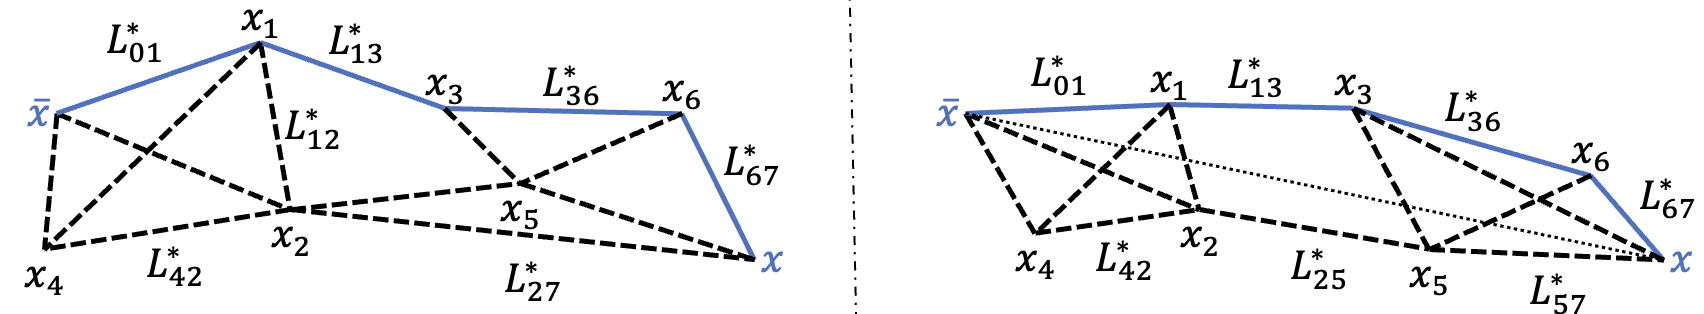
\includegraphics[width=0.9\textwidth]{figures/method.png}}
\caption{\textbf{Method overview.} For an input $\textbf{x}$, a baseline $\overline{\textbf{x}}$, and a set of points $\textbf{x}_i$, we compute the kNN graph using the euclidean distance (dashed lines). For each couple $(\textbf{x}_i, \textbf{x}_j)$, we then compute the integrated gradients $\textrm{L}^*_{ij}$ using Equation \ref{eq:log_geo_approx}. For clarity, not all $\textrm{L}^*_{ij}$ are present on the figure. 0 and 7 represent $\overline{\textbf{x}}$ and $\textbf{x}$ respectively. Using the resulting undirected weighted graph, we use the Dijkstra algorithm to find the shortest path between $\textbf{x}$ and $\overline{\textbf{x}}$ (blue continuous lines). On the left, the points $\textbf{x}_i$ are provided while, on the right, the points are generated along the straight line between $\textbf{x}$ and $\overline{\textbf{x}}$ (dotted line).}
\label{fig:method}
\end{center}
\vskip -0.2in
\end{figure*}

\paragraph{Assumption of the approximation.} 

Here we formalise the intuition that, for a pair of neighbours, the geodesic path between them is close to the euclidean one. Notice that the derivative of the neural network $f$ is Lipschitz continuous,

\begin{equation}
    \exists \textrm{K} \, \forall \textbf{x}, \textbf{y}, \, ||\textrm{J}_{\textbf{x}} - \textrm{J}_{\textbf{y}}|| \leq \textrm{K} \times ||\textbf{x} - \textbf{y}||.
\label{eq:deriv_lip}
\end{equation}

Equation \ref{eq:deriv_lip} is equivalent to the Hessian of $f$ being bounded. Under this assumption, if two points $\textbf{x}$ and $\textbf{y}$ are close enough, the Jacobian of one point is approximately equal to the other: if $||\textbf{x} - \textbf{y}|| \le \epsilon$, then $\textrm{J}_{\textbf{x}} \approx \textrm{J}_{\textbf{y}}$. As a result, the length between $\textbf{x}$ and $\textbf{y}$, for a curve $\gamma$, is: $\textrm{L}(\gamma) \approx \int_{\gamma} ||\textrm{J}_{\textbf{x}}|| \, d\textbf{x} \approx ||\textrm{J}_{\textbf{x}}|| \int_{\gamma} d\textbf{x}$. Due to the triangular inequality, the shortest path $\gamma^*$ is then a straight line, and we have: $\textrm{L}^*(\textbf{x}, \textbf{y}) \approx ||\textrm{J}_{\textbf{x}}|| \times ||\textbf{x} - \textbf{y}||$.

As a result, under this assumption, if two points are close, the geodesic path can be approximated with a straight line. Note that even though we take the path between two neighbouring points to be a straight line, we do not assume that the Jacobian of the function between the two points is constant. 

\paragraph{Handling disconnected graphs}

An issue with the graph computed with the kNN algorithm is that it could be disconnected, in which case it could be impossible to compute a path between an input and a baseline. To alleviate this issue, we add so called ``bridges'' to the graph, as following: for each disconnected component, we add one link between them, specifically between two points of each component having the lowest euclidean distance. An illustration of this method is displayed on Figure \ref{fig:bridge}.

\begin{figure}[ht]
\vskip 0.2in
\begin{center}
\centerline{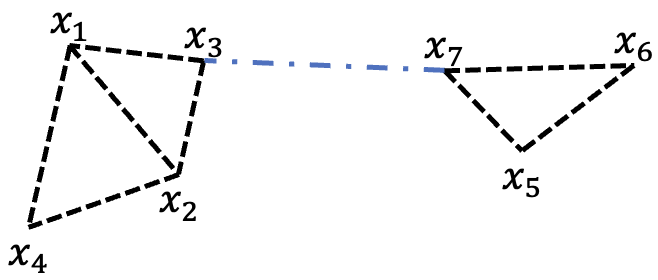
\includegraphics[width=0.8\columnwidth]{figures/bridge.png}}
\caption{When the kNN graph is disconnected, as illustrated here, it would be impossible to compute Geodesic IG between certain points, for instance $\textbf{x}_1$ and $\textbf{x}_5$ here. To solve this, we add a single link between disconnected graphs, here between $\textbf{x}_3$ and $\textbf{x}_7$.}
\label{fig:bridge}
\end{center}
\vskip -0.2in
\end{figure}

However, we stress that this solution is not optimal, and argue that a better way of handling this issue would be to avoid disconnected graphs in the first place. This can be done by increasing the number of neighbours k.

\subsection{Approximation of the geodesic with energy-based sampling.}
While our $k$NN-based method is effective for explaining simpler models, its applicability diminishes as model complexity increases. In such cases, a prohibitively large number of samples is required between the baseline and the input to provide accurate estimates of the geodesic path. Even with relatively large number of samples, it is not trivial where on the manifold to sample the points to adequately capture the gradient landscape. Furthermore, once the points are sampled, searching the graph for the shortest path will be computationally too intensive. For such use-cases, we devise another approximation procedure based on an energy-base sampling method, such as Stochastic Variational Inference (SVI).

As we observed in Remark \ref{rem:shortest}, we would like to sample from the shortest paths between two points on the input space that avoids high gradient regions as much as possible. Therefore, we want to deviate from the straight line to avoid high gradient regions. This process can be approximated in the following way. First we start with a straight line between the two points and define a potential energy as a combination of two terms. One for the distance of the path to be optimised to the straight line,  and the other is a curvature penalty term. Finding the minimum energy path, therefore samples approximately on the geodesic lines. More formally, let us define the distance term: $d(x,y) := |x-y|_2$, and the curvature term: $c(x):=|\nabla f(x)|_2$ where $f$ is the neural network. The total energy being minimised is

\begin{equation}
E(\gamma) = \sum_{i=1}^{n} \|\gamma_i - \gamma^0_i\|_2 - \beta\|\nabla f(\gamma_i)\|_2, 
\end{equation}
where $\gamma$ is the path $\gamma^0$ is the initial path $beta$ controls trade-off between distance and curvature.

With this energy function, one can use a suitable sampling method, such as SVI or Hamiltoniam Monte Carlo to sample points on the geodesic paths. Here we briefly describe the SVI optimisation, as this has a good balance of computational efficiency and accuracy.

SVI provides a probabilistic framework for optimising paths between input and baseline points. To achieve this, SVI defines a probability distribution $p(\gamma|\gamma_0)$ proportional to $exp(-E(\gamma))$, where $E(\gamma)$ is our defined potential energy. Rather than directly sampling from this complex distribution, we introduce a simpler variational distribution $q(\gamma)$ parameterised by learnable means and scales. This guide distribution takes the form of a factorised normal distribution $\prod_i N(\mu_i,\sigma_i)$ over path deviations.

The optimisation proceeds by minimising the KL divergence between $q(\gamma)$ and the true posterior through maximisation of the Evidence Lower Bound (ELBO). Critically, this allows us to learn optimal parameters for $q(\gamma)$ through gradient-based optimisation. The learned means $\mu_i$ define the optimal path deviations from the initial straight-line path, while the scales $\sigma$ capture uncertainty in these deviations. This probabilistic approach naturally samples of the low-energy regions.

We use this method in our computer vision experiments and show its efficacy in section \label{sec:experiments}. However here we find it instructive to visualise these paths on the 2D example of half-moons, Fig. \ref{fig:svi_moons}, even though for simpler use-cases such as this we would prefer the $k$NN method, as they are easier to control. 

\begin{figure}[ht]
	\vskip 0.2in
	\begin{center}
		\centerline{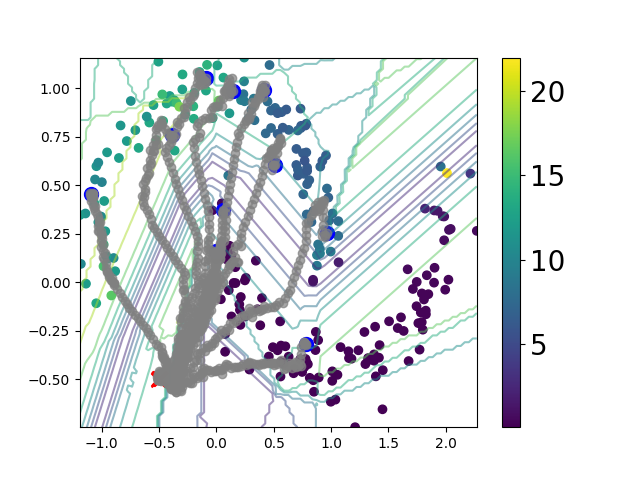
\includegraphics[width=0.95\columnwidth]{figures/svi_ig_moons.png}}
		\caption{\textbf{Visualising 10 random paths.} For a simple case of half-moons with 1000 samples, we show the sampled paths between 10 pairs of points. As we see on low gradient regions the sampler prefers straigh lines, whereas in high gredient regions the path becomes closer to perpendicular to the large gradient vectors to cross the region as quickly as possible.}
		\label{fig:svi_moons}
	\end{center}
	\vskip -0.2in
\end{figure}

\subsection{Axiomatic properties}

\paragraph{Symmetry preserving of Geodesic IG}

The family of generalisations of Integrated Gradients to non-straight paths, such as Eq. \ref{eq:geodesic_ig}, is called \emph{path methods} of explanation. We see in \citet{sundararajan2017axiomatic} that all path methods satisfy all of the axioms that IG is based on, apart from the symmetry axiom that we discussed in the introduction. \citet[Theorem 1]{sundararajan2017axiomatic} shows that Integrated Gradients is the only path-method on Euclidean surfaces that is symmetry preserving. Here we demonstrate that Geodesic Integrated Gradients satisfies symmetry property on Riemannian manifolds, and it is the only path-based method that does so. 

Let the $i$th and $j$th dimensions of $\gamma(t)$ be $\gamma_i(t)$ and $\gamma_j(t)$ respectively and $f$ be a function differentiable almost everywhere on $t$. Furthermore, take $f$ to be symmetric with respect to $x_i$ and $x_j$. If $\gamma_i(t) = \gamma_j(t)$ for all $t \in [0,1]$, then we have 
\begin{equation}
	\begin{split}
		& ||\partial_t f(\gamma_i(t)) \times \dot\gamma_i(t)|| = ||\partial_t f(\gamma_j(t)) \times \dot\gamma_j(t)||,
	\end{split}
	\label{eq:norms}
\end{equation}
almost everywhere on $t$. Therefore, the $i$th and $j$th components of Eq. \ref{eq:length} are equal. Furthermore, since  Eq. \ref{eq:geodesic_ig} integrates along the path that is an approximation of Eq. \ref{eq:length}, we have $\textrm{Geodesic IG}_i = \textrm{Geodesic IG}_j$. Indeed our geodesic paths satisfy  $\gamma_i(t) = \gamma_j(t)$ for all $t \in [0,1]$ on the Riemannian manifolds. To see this, let us select a baseline $\overline{\textbf{x}}$ and $U$ a Riemann neighbourhood centred at $\overline{\textbf{x}}$. Let us also define the geodesic path $\gamma$ such as $\gamma(0) = \overline{\textbf{x}}$. Further, define $\textbf{v}(t):=\gamma'(t)$, where $\gamma'$ is the derivative of $\gamma$. Then, in the local coordinates system of the neighbourhood of any point, called normal coordinates, we have $\gamma(t) = (tv_1(t), ..., tv_n(t))$. Since the function is symmetric in the $i$th and $j$th dimensions, we have $v_i$ and $v_j$ are the same everywhere. From this, we can see that $\gamma_i(t) = \gamma_j(t)$ for all $t \in [0,1]$ and therefore Geodesic IG satisfies symmetry. In other words, since the geodesic generalises straight paths to Riemannian manifolds, it follows that the symmetry property of IG on Euclidean space is extended to Geodesic IG on Riemannian manifolds. In fact, using the same argument as above, the proof of \citet[Theorem 1]{sundararajan2017axiomatic} can be readily used to show that Geodesic IG is the only path method on Riemannian manifolds that satisfy symmetry.

, including symmetry. The symmetry axiom is defined in the following way. 
\begin{definition}
	Consider an input-baseline pair $\textbf{x}$ and $\overline{\textbf{x}}$, and a function $f$ that is symmetric in dimensions $i$ and $j$. If $\textbf{x}_i = \textbf{x}_j$ and $\overline{\textbf{x}}_i = \overline{\textbf{x}}_j$, then an attribution method is Symmetry-Preserving if $attr_i(\textbf{x}; f) = attr_j(\textbf{x}; f)$, where $attr_n(\textbf{x}; f)$ is the attribution of $\textbf{x}_n$.
\end{definition}
\citep[Theorem 1]{sundararajan2017axiomatic} shows that IG is the only path method that satisfies symmetry on Euclidean space. We generalise this theorem for Geodesic IG on Riemannian manifolds.
\section{Experiments}
\label{sec:experiments}

To validate our method, we performed experiments on two datasets: one is the synthetic half-moons dataset, and the other is the real-world Pascal VOC 2012 dataset.

\subsection{Experiments on the half-moons dataset}
\label{subsec:half-moons}

Here we give the details of the half-moons experiment discussed in the Introduction section. We use the half-moons dataset provided by Scikit learn \citep{scikit-learn} to generate 10,000 points with a Gaussian noise of $\mathcal{N}(0, 0.2)$. The dataset is split into 8,000 training points and 2,000 testing ones. The model used is an MLP.

We measure two indicators of performance for each attribution method: a lack of artifacts not reflecting the model's behaviour, and a low variation of attributions between close points. To that goal, we use two metrics, \textbf{purity} and \textbf{standard deviation}, defined in the following way. We know that a well-trained model should classify about half of the data points as upper moon, class $1$, and the other half as lower moon, class $0$. Such a model should consider both features of each point important for the classification into class $1$. Therefore, for such a model, we expect in a good attribution method, the top $50\%$ points as ranked by the quantity $\widetilde{attr}(\textbf{x}; f) = \sum_{i=0}^1 |attr_i(\textbf{x}; f)|$, to be classified as $1$ (assuming the baseline is chosen as a point to which the network gives a near-zero score). With this in mind, purity is defined as
\begin{equation}
\begin{split}
    \textrm{Purity} &= \frac{1}{N/2}\sum_{\textbf{x}, \, \widetilde{attr}(\textbf{x}; f) \in \textrm{Top 50\% of all attr}} \textrm{argmax}(f(\textbf{x})),
\end{split}
\label{eq:moons-purity}
\end{equation}
where $N$ is the number of data points. We see that this is the average value of the predicted class labels for half of the points. From the above, we infer that, for a well-trained model, we prefer an attribution method that results in the purity close to $1$. In contrast, a random attribution method in this case would result in the purity score of $0.5$. 

For the second metric, standard deviation, points that belong to the same moon to have similar $\widetilde{attr}(\textbf{x}; f)$. Therefore, define
\begin{equation}
\begin{split}
    \textrm{Std}_i &= \textrm{std}\{\widetilde{attr}(\textbf{x}; f), \, \textrm{argmax}(f(\textbf{x})) \in \textrm{Moon }_i\}.
\end{split}
\label{eq:moons-std}
\end{equation}
We expect this standard deviation metric to be low for the points belonging to either class. 

In this experiment, we compare the results of attributions from Geodesic IG with the original IG, as well as more recent comparable methods including Enhanced IG \citep{jha2020enhanced}, GradientShap \citep{lundberg2017unified}, SmoothGrad \citep{smilkov2017smoothgrad}.

For all of the methods, we use $(-0.5, -0.5)$ as a baseline. Enhanced IG is an improvement over IG where the kNN algorithm is used to avoid computing gradients on paths on out of sample distributions. The chosen number of neighbours for the kNN part of both Enhanced IG and Geodesic IG is $5$. We perform an ablation study of this parameter in Appendix \ref{app:half-moons}. 

\begin{table}[t]
	\centering
	\resizebox{0.48\textwidth}{!}{%
	\begin{tabular}{lccc}
		\toprule
		\textbf{Method} & Purity $\uparrow$ & $\textrm{STD}_0$ $\downarrow$ & $\textrm{STD}_1$ $\downarrow$ \\
		\midrule
        GradientShap    & 0.761 (0.158)   & 1.90 (0.520)  & 5.01 (0.581) \\
		IG              & 0.802 (0.142)  & 1.44 (0.139) & 4.915 (0.574)  \\
        SmoothGrad      & 0.800 (0.142)  &  1.42 (0.139) & 4.720 (0.649)  \\
        Enhanced IG     & 0.738 (0.209)  &  1.23 (0.229) & 1.876 (1.10) \\
		\midrule
		Geodesic IG     & \textbf{0.978} (0.0143)  & \textbf{0.237} (0.0278) & \textbf{0.267} (0.129) \\
		\bottomrule
	\end{tabular}%
	}
	\caption{Evaluation of different attribution methods on a half-moons dataset with Gaussian noise $\mathcal{N}(0, 0.2)$. The results over 5 different seeds are averaged, with the corresponding standard deviation in brackets. We present in Appendix \ref{app:half-moons} more results with different amounts of Gaussian noise.}
	\label{tab:results_moons_2}
\end{table}

The quantitative analysis of the results are given in Table \ref{tab:results_moons_2}, where we see that Geodesic IG significantly outperforms all other methods on all metrics. In particular, notice that all other methods perform relatively poorly on STD$_1$. This is because for this metric, the integration path has to cross the decision boundary. However, the other methods might cross the decision boundary differently and regardless of the function's gradient, resulting in spuriously different attributions for different points belonging to class $1$. In Appendix \ref{app:half-moons} we see that the gap between the performance of geodesic IG and the other methods increases as the Gaussian noise of the half-moons increases. To provide better understanding of these results we present more analysis on this dataset in Section \ref{sec:related_work}.

\subsection{Experiments on the Pascal VOC 2012 dataset}
\label{subsec:voc}

\begin{figure*}[ht]
\vskip 0.2in
\begin{center}
\centerline{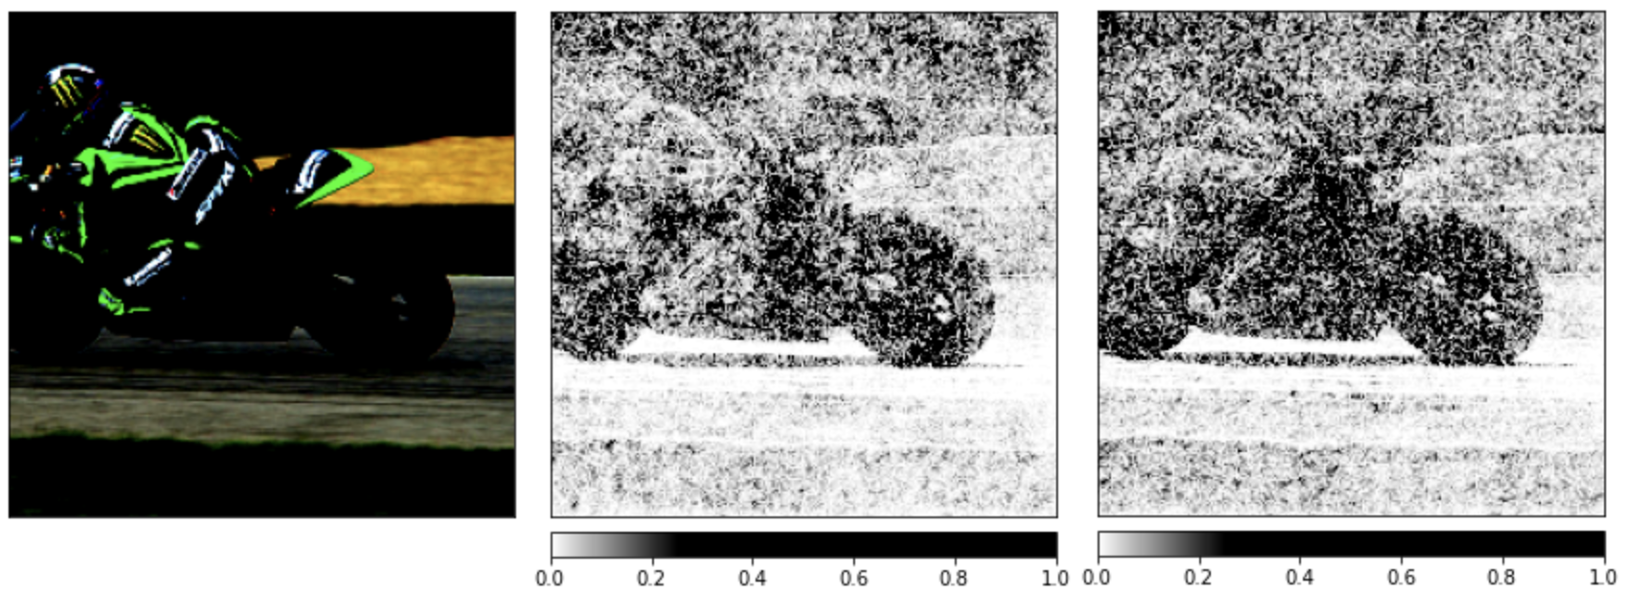
\includegraphics[width=0.9\textwidth]{figures/images.png}}
\caption{Comparison between Integrated Gradients and Geodesic IG on one image. The predicted class is ``motor-scooter". The left figure is the original image, while the other two are heatmaps of respectively the IG (center) and the Geodesic IG (right). We can see that our method seems to reduce the amount of noise and is able to provide a sharper heatmap, compared with the vanilla IG. More comparisons are presented in Appendix \ref{app:voc}.}
\label{fig:qualitative-comp}
\end{center}
\vskip -0.2in
\end{figure*}

Now we would like to test our method on a real-world dataset. To this aim, we use the Pascal VOC 2012 dataset, which consists of labelled images \citep{pascal-voc-2012}. We also use a pre-trained ResNet model to generate predictions to be explained \citep{he2016deep}. We also perform the analysis on 100 randomly sampled images from the test set.

We compare our method with various baselines: Integrated Gradients, GradientShap, SmoothGrad, InputXGradients \citep{shrikumar2016not}, Lime \citep{ribeiro2016should}, KernelShap \citep{lundberg2017unified}, Occlusion \citep{zeiler2014visualizing} Augmented Occlusion \citep{tonekaboni2020went} and Enhanced IG \citep{jha2020enhanced}.

For both Enhanced IG and Geodesic IG, as the VOC dataset is high-dimensional, we generate points of the graph following the method described in our Method section, using the straight line as a guide. The baseline is chosen here as a uniformly black image. As with the half-moons dataset, we use 5 neighbours for the kNN algorithm.

To evaluate the performance of an attribution method, we use here 3 different metrics:

\begin{itemize}
    \item \textbf{Comprehensiveness} \citep{deyoung2019eraser}: We mask the top k\% most important features in absolute value, and compute the average change of the predicted class probability compared with the original image. A higher score is better as it indicates masking these features results in a large change of predictions.
    \item \textbf{Sufficiency} \citep{deyoung2019eraser}: We only keep the top k\% most important features in absolute value, and compute the average change of the predicted class probability compared with the original image. A lower score is better as it means that these important features are sufficient to retain similar predictions.
    \item \textbf{Log-odds}\footnote{This metric should be called \emph{Log-probabilities}. However, since Log-odds is a commonly used name in the literature, we refer to it as Log-odds.} \citep{shrikumar2017learning}: We mask the top k\% most important features in absolute value, and measure the negative logarithmic probabilities on the predicted class compared with the original one. Lower scores are better.
\end{itemize}

\begin{table}[t]
	\centering
	\resizebox{0.48\textwidth}{!}{%
	\begin{tabular}{lccc}
		\toprule
		\textbf{Method} & Comp $\uparrow$ & Suff $\downarrow$ & LO $\downarrow$ \\
		\midrule
        Input X Gradients   & 0.360 (0.0280) & 0.545 (0.0254) & -2.66 (0.167)  \\
        GradientShap        & 0.425 (0.0130) & 0.544 (0.0260) & -3.28 (0.164)  \\
		IG                  & 0.427 (0.0072) & 0.544 (0.0254) & -3.31 (0.117)  \\
        SmoothGrad          & 0.404 (0.0160) & 0.536 (0.0263) & -3.09 (0.222)  \\
        Lime                & 0.197 (0.0139) & 0.529 (0.0176) & -1.31 (0.082)  \\
        Kernel Shap         & 0.193 (0.0179) & \textbf{0.527} (0.0172) & -1.30 (0.114) \\
        Occlusion           & 0.340 (0.0263) & 0.534 (0.0211) & -2.26 (0.061) \\
        Aug Occlusion       & 0.352 (0.0177) & 0.540 (0.0235) & -2.37 (0.118) \\
        Enhanced IG         & 0.445 (0.0104) & 0.543 (0.0264) & -3.75 (0.125) \\
		\midrule
		Geodesic IG         & \textbf{0.449} (0.0107) & 0.543 (0.0261) & \textbf{-3.77} (0.168) \\
		\bottomrule
	\end{tabular}%
	}
	\caption{Evaluation of different attribution methods on 100 randomly sampled images from the Pascal VOC test set. The metrics are computed by removing or keeping the top 5\% most important features. More results are provided in Appendix \ref{app:voc}.}
	\label{tab:results_voc}
\end{table}

Figure \ref{fig:qualitative-comp} provides a qualitative comparison between Geodesic IG and Integrated Gradients, while Table \ref{tab:results_voc} provides a quantitative comparison between Geodesic IG and various other methods. The analysis shows that Geodesic IG is a very powerful method in explaining the model's behavior on the dataset. Table \ref{tab:results_voc} shows that for this dataset, Geodesic IG outperforms almost all other methods in terms of comprehensiveness and log-odds, and is on par with Enhanced IG. However, as we further discuss in section \ref{sec:related_work}, the path of Enhanced IG does not take the model's gradients into account, potentially leading to significant artefacts, and lacks a straightforward way for improvement. On the other hand, Geodesic IG could be further improved by deriving better approximations of the geodesic path, which we discuss in section \ref{sec:method}. In this experiment, we have indeed used the simple `guide' method according to Eq. \ref{eq:guide}, and we expect that a more sophisticated approximation method would further improve the results.

Furthermore, the Sufficiency results in Table \ref{tab:results_voc} do not seem to discriminate between different explanation methods. However, in Appendix \ref{app:voc} we present more results, in which Geodesic IG outperforms the original IG on this metric.

\section{Related Work}
\label{sec:related_work}

Approximating geodesic paths is a widely studied area of research, and many methods to do so have been developed. For a comprehensive survey on this subject, please refer to \citet{crane2020survey}. Our work is specifically inspired from the ISOMAP method \citep{tenenbaum2000global}, a dimensionality reduction method which approximates geodesic paths on a manifold. However, our method differs from ISOMAP in that we weight our graph not using euclidean distance, but the norms of a model's gradients. Our aim is indeed not to model the input space, but to explain a neural network by building paths avoiding high-gradients regions.

As mentioned in Section \ref{sec:experiments}, the idea of using a $k$NN algorithm to avoid computing gradients on out of distribution data points has also been used in Enhanced Integrated Gradients \citet{jha2020enhanced}. However, this method creates a path which is model agnostic, as it does not necessarily avoid high gradients regions. As a result, it can lead to significant artefacts which do not reflect the model's behaviour. To support this argument, we provide an example where this method fails on the half-moons datasets (Figure \ref{fig:enhanced_ig}). 

\begin{figure}[ht]
\vskip -0.2in
\begin{center}
\centerline{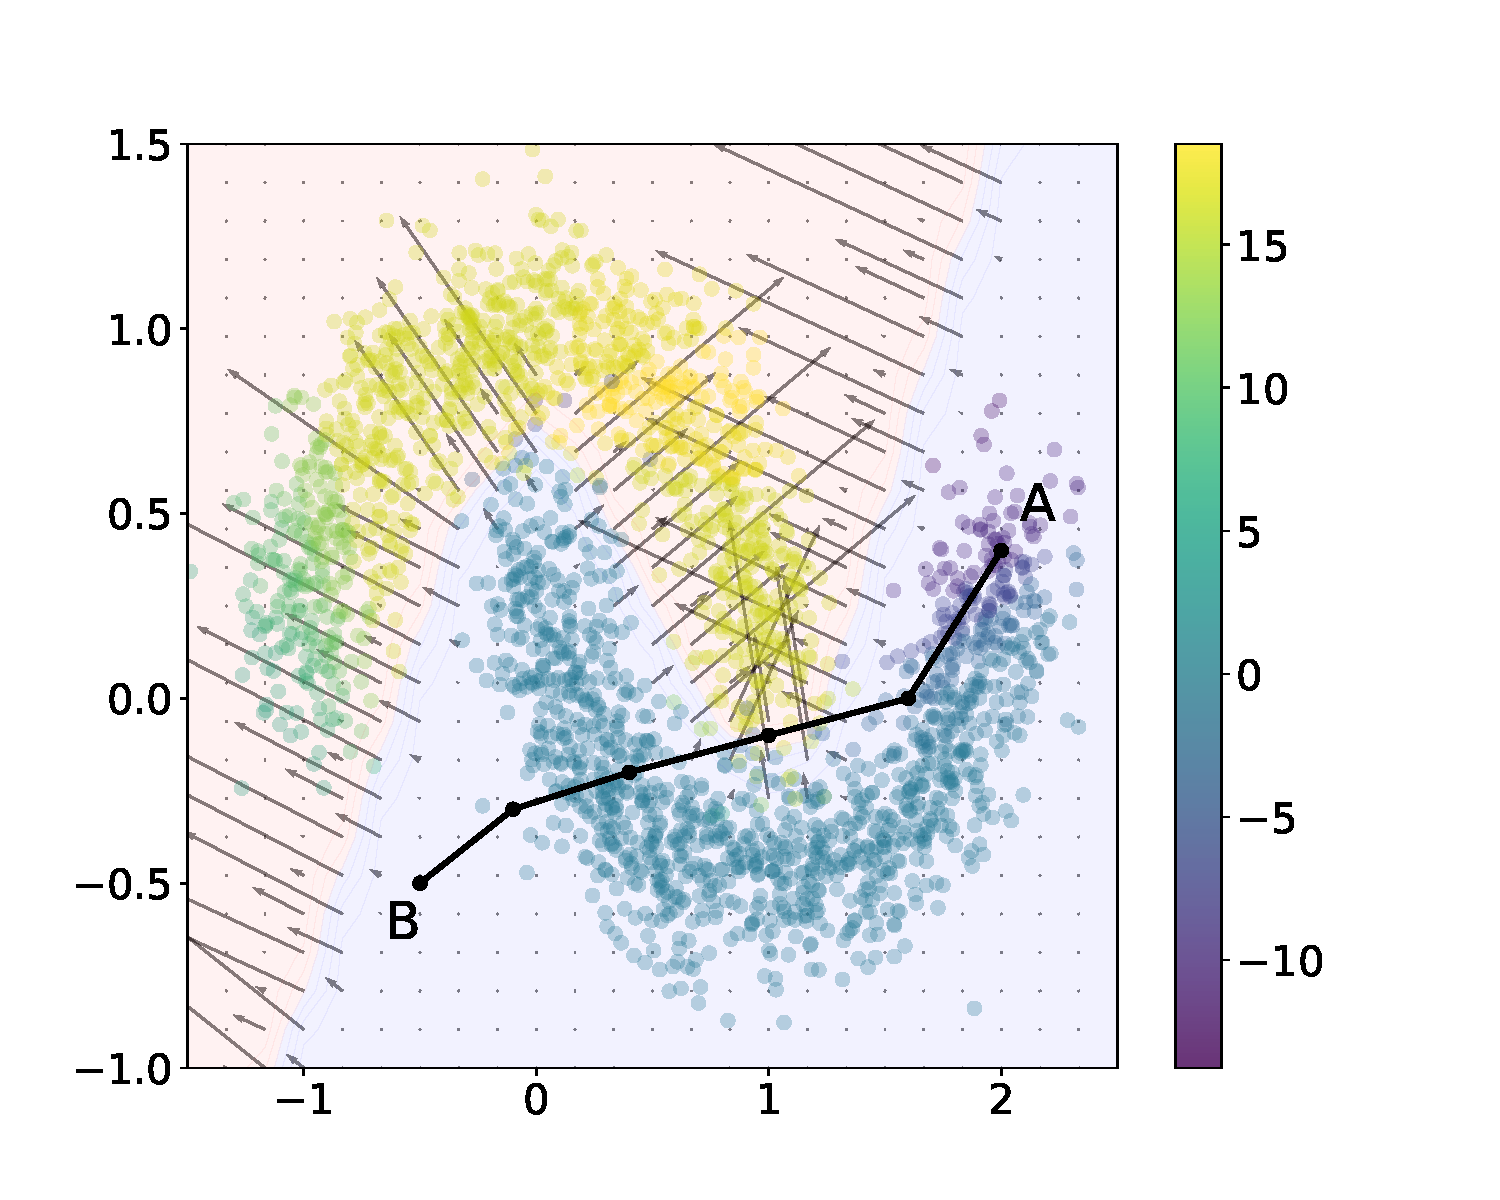
\includegraphics[width=\columnwidth]{figures/enhanced_ig_y.pdf}}
\caption{\textbf{Enhanced IG attributions.} Enhanced IG computes a $k$NN algorithm, uses Dijsktra to find the shortest path between an input and a reference baseline, and computes gradients along this path. However, this method is model agnostic and can as a result cross a high gradients region, which is the case in this example, between the input A and the baseline B. Input A therefore has a high attribution which does not reflect the model's true behavior. In this example, the noise is $\mathcal{N}(0, 0.15)$.}
\label{fig:enhanced_ig}
\end{center}
\vskip -0.2in
\end{figure}

The idea of adapting the path according to the model has be proposed by \citet{kapishnikov2021guided}, calling their method Guided Integrated Gradients. Their method computes this path greedily by selecting around 10\% of the features that have the lowest absolute value of the partial derivatives, and switching these features from the baseline's values to the input's values. However, as the authors indicate, such method can create out of distribution data points, with part of their features either matching the input or the baseline. As a result, they add a hyperparameter K, which forces the path to go through K points along the straight line between the input and the baseline. 
We argue, however, that, by directly approximating the path of least resistance, our method is more principled compared to Guided IG. In Guided IG, it is not clear how to choose the value of K: a too low value could create out of distribution samples, while a too high one would force the path to be close to the straight line and potentially cross high gradients regions. It is similarly not clear why switching 10\% of the features, and how to tune this hyperparamer. On the other hand, we argue that Geodesic IG does not have this issue. It has indeed two hyperparamers: the number of points used to approximate the geodesic path, and the number k of nearest neighbours. Yet, the performance of Geodesic IG should improve when both hyperparamers values increase, as, when more points or more neighbours are used, the approximation of the geodesic path should improve. Increasing these values would, however, require more computing and performance needs to be balanced with the amount of compute available.
\section{Discussion}
\label{sec:discussion}

We have identified in this paper potential issues with path-based attribution methods: the presence of artefacts due to ignoring the curvatures of the model. To overcome these issues, we have introduced Geodesic Integrated Gradients, an adaptation of the original IG method which integrates gradients not along a straight line, but along the geodesic of a manifold defined by the model.

By avoiding high-gradients regions in the input space, we have shown that Geodesic IG can successfully address these issues. Moreover, it follows all of the axioms defined by \citet{sundararajan2017axiomatic}. 

We have presented two methods to approximate these geodesic paths: one based on $k$NN and the other Stochastic Variational Inference. Whilst our method shows clear advantage over the alternatives, evaluated by metrics such as Comprehensiveness and Log-Odds, there are some further research questions that we leave for future explorations. One is around computational intensiveness of our methods, as we discussed in section \ref{sec:experiments}. The other is the inherent noise in any sampling process that we may wish to use for approximating the geodesic lines. Regarding the noise, it is concievable that a method involving directly solving the geodesic equation might result in less noisy approximation of the geodesic paths. Depending on the way one solves such equations, it is possible that finding the geodesic paths might become more computationally efficient than using SVI. 
% \section{Acknowledgements}
\label{acknowledgements}

This is the acknowledgements section.

% In the unusual situation where you want a paper to appear in the
% references without citing it in the main text, use \nocite
\nocite{langley00}

\bibliography{bib}
\bibliographystyle{icml2023}


%%%%%%%%%%%%%%%%%%%%%%%%%%%%%%%%%%%%%%%%%%%%%%%%%%%%%%%%%%%%%%%%%%%%%%%%%%%%%%%
%%%%%%%%%%%%%%%%%%%%%%%%%%%%%%%%%%%%%%%%%%%%%%%%%%%%%%%%%%%%%%%%%%%%%%%%%%%%%%%
% APPENDIX
%%%%%%%%%%%%%%%%%%%%%%%%%%%%%%%%%%%%%%%%%%%%%%%%%%%%%%%%%%%%%%%%%%%%%%%%%%%%%%%
%%%%%%%%%%%%%%%%%%%%%%%%%%%%%%%%%%%%%%%%%%%%%%%%%%%%%%%%%%%%%%%%%%%%%%%%%%%%%%%
\newpage
\appendix
\onecolumn
\section{Additional Half-moons results}
\label{app:half-moons}

We present on Figure \ref{fig:noises} more results on the half-moons dataset, using different amounts of noise. We can see that, for certain amount of noise, Enhanced IG dramatically fails, while Geodesic IG performs consistently well on every amount of noise tested here. We believe that the failure of Enhanced IG in the high-noise setting is due to the following reason. As noise increases the points on either moons get closer to each other. As a result, the model loses the property that gradients are only large on the decision boundary and fall rapidly as we move away. Therefore a lot of points are on the high-gradient regions. However, Enhanced IG chooses the path purely based on nearest neighbours, ignoring model gradients. Hence, leading to low purity. This is contrast to geodesic IG, which actively avoids regions of high gradients.

\begin{figure}[ht]
\vskip 0.2in
\begin{center}
\centerline{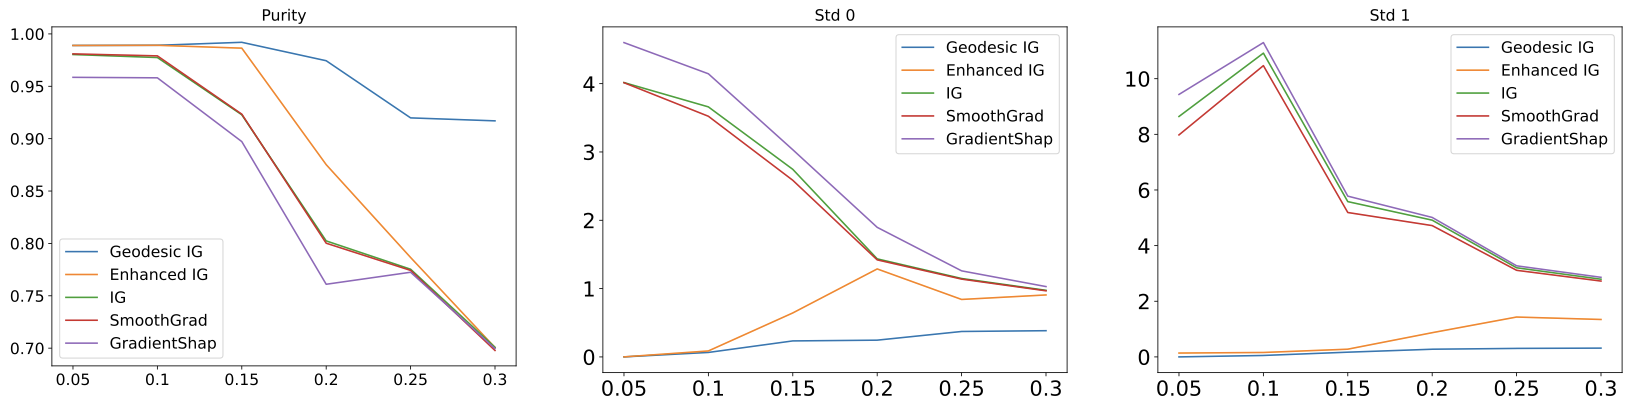
\includegraphics[width=0.9\textwidth]{figures/noises.png}}
\caption{Evaluation of different attribution methods on the half-moons dataset with different amounts of noise: $\mathcal{N}(0, x)$ where $x$ is defined as the axis of each plot.}
\label{fig:noises}
\end{center}
\vskip -0.2in
\end{figure}

We also perform here an ablation study using different values of k for the kNN algorithm. We show the results on Figure \ref{fig:knn}. The results show that increasing $k$ harms the performance of Enhanced IG, leaving the ones of Geodesic IG unchanged. This is probably due to the fact that increasing k allows connections between points further apart, potentially crossing high-gradients regions. While Geodesic IG would not follow such paths, Enhanced IG only uses euclidean distance, and is therefore more likely to generate paths crossing high-gradients regions.

\begin{figure}[ht]
\vskip 0.2in
\begin{center}
\centerline{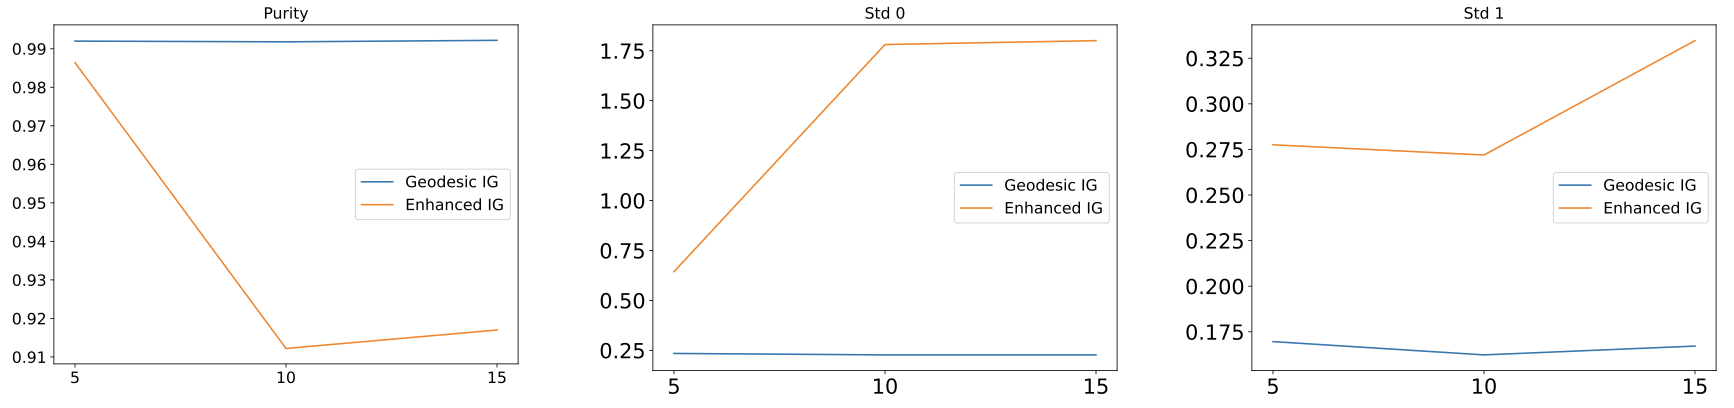
\includegraphics[width=0.9\textwidth]{figures/knn.png}}
\caption{Evaluation of Geodesic IG and Enhanced IG for different values of k in the kNN algorithm. We can see that increasing this parameter harms Enhanced IG performance, while it does not seem to have a major effect on Geodesic IG performance.}
\label{fig:knn}
\end{center}
\vskip -0.2in
\end{figure}

\newpage

\section{Additional heatmaps and results on Pascal VOC 2012}
\label{app:voc}

We also qualitatively compare on Figure \ref{fig:more_images} Geodesic IG with the original IG on 5 different images of the Pascal VOC 2012 dataset. Geodesic IG heatmaps appears to be less blurry than the ones generated with original IG method.

\begin{figure}[ht]
\vskip 0.2in
\begin{center}
\centerline{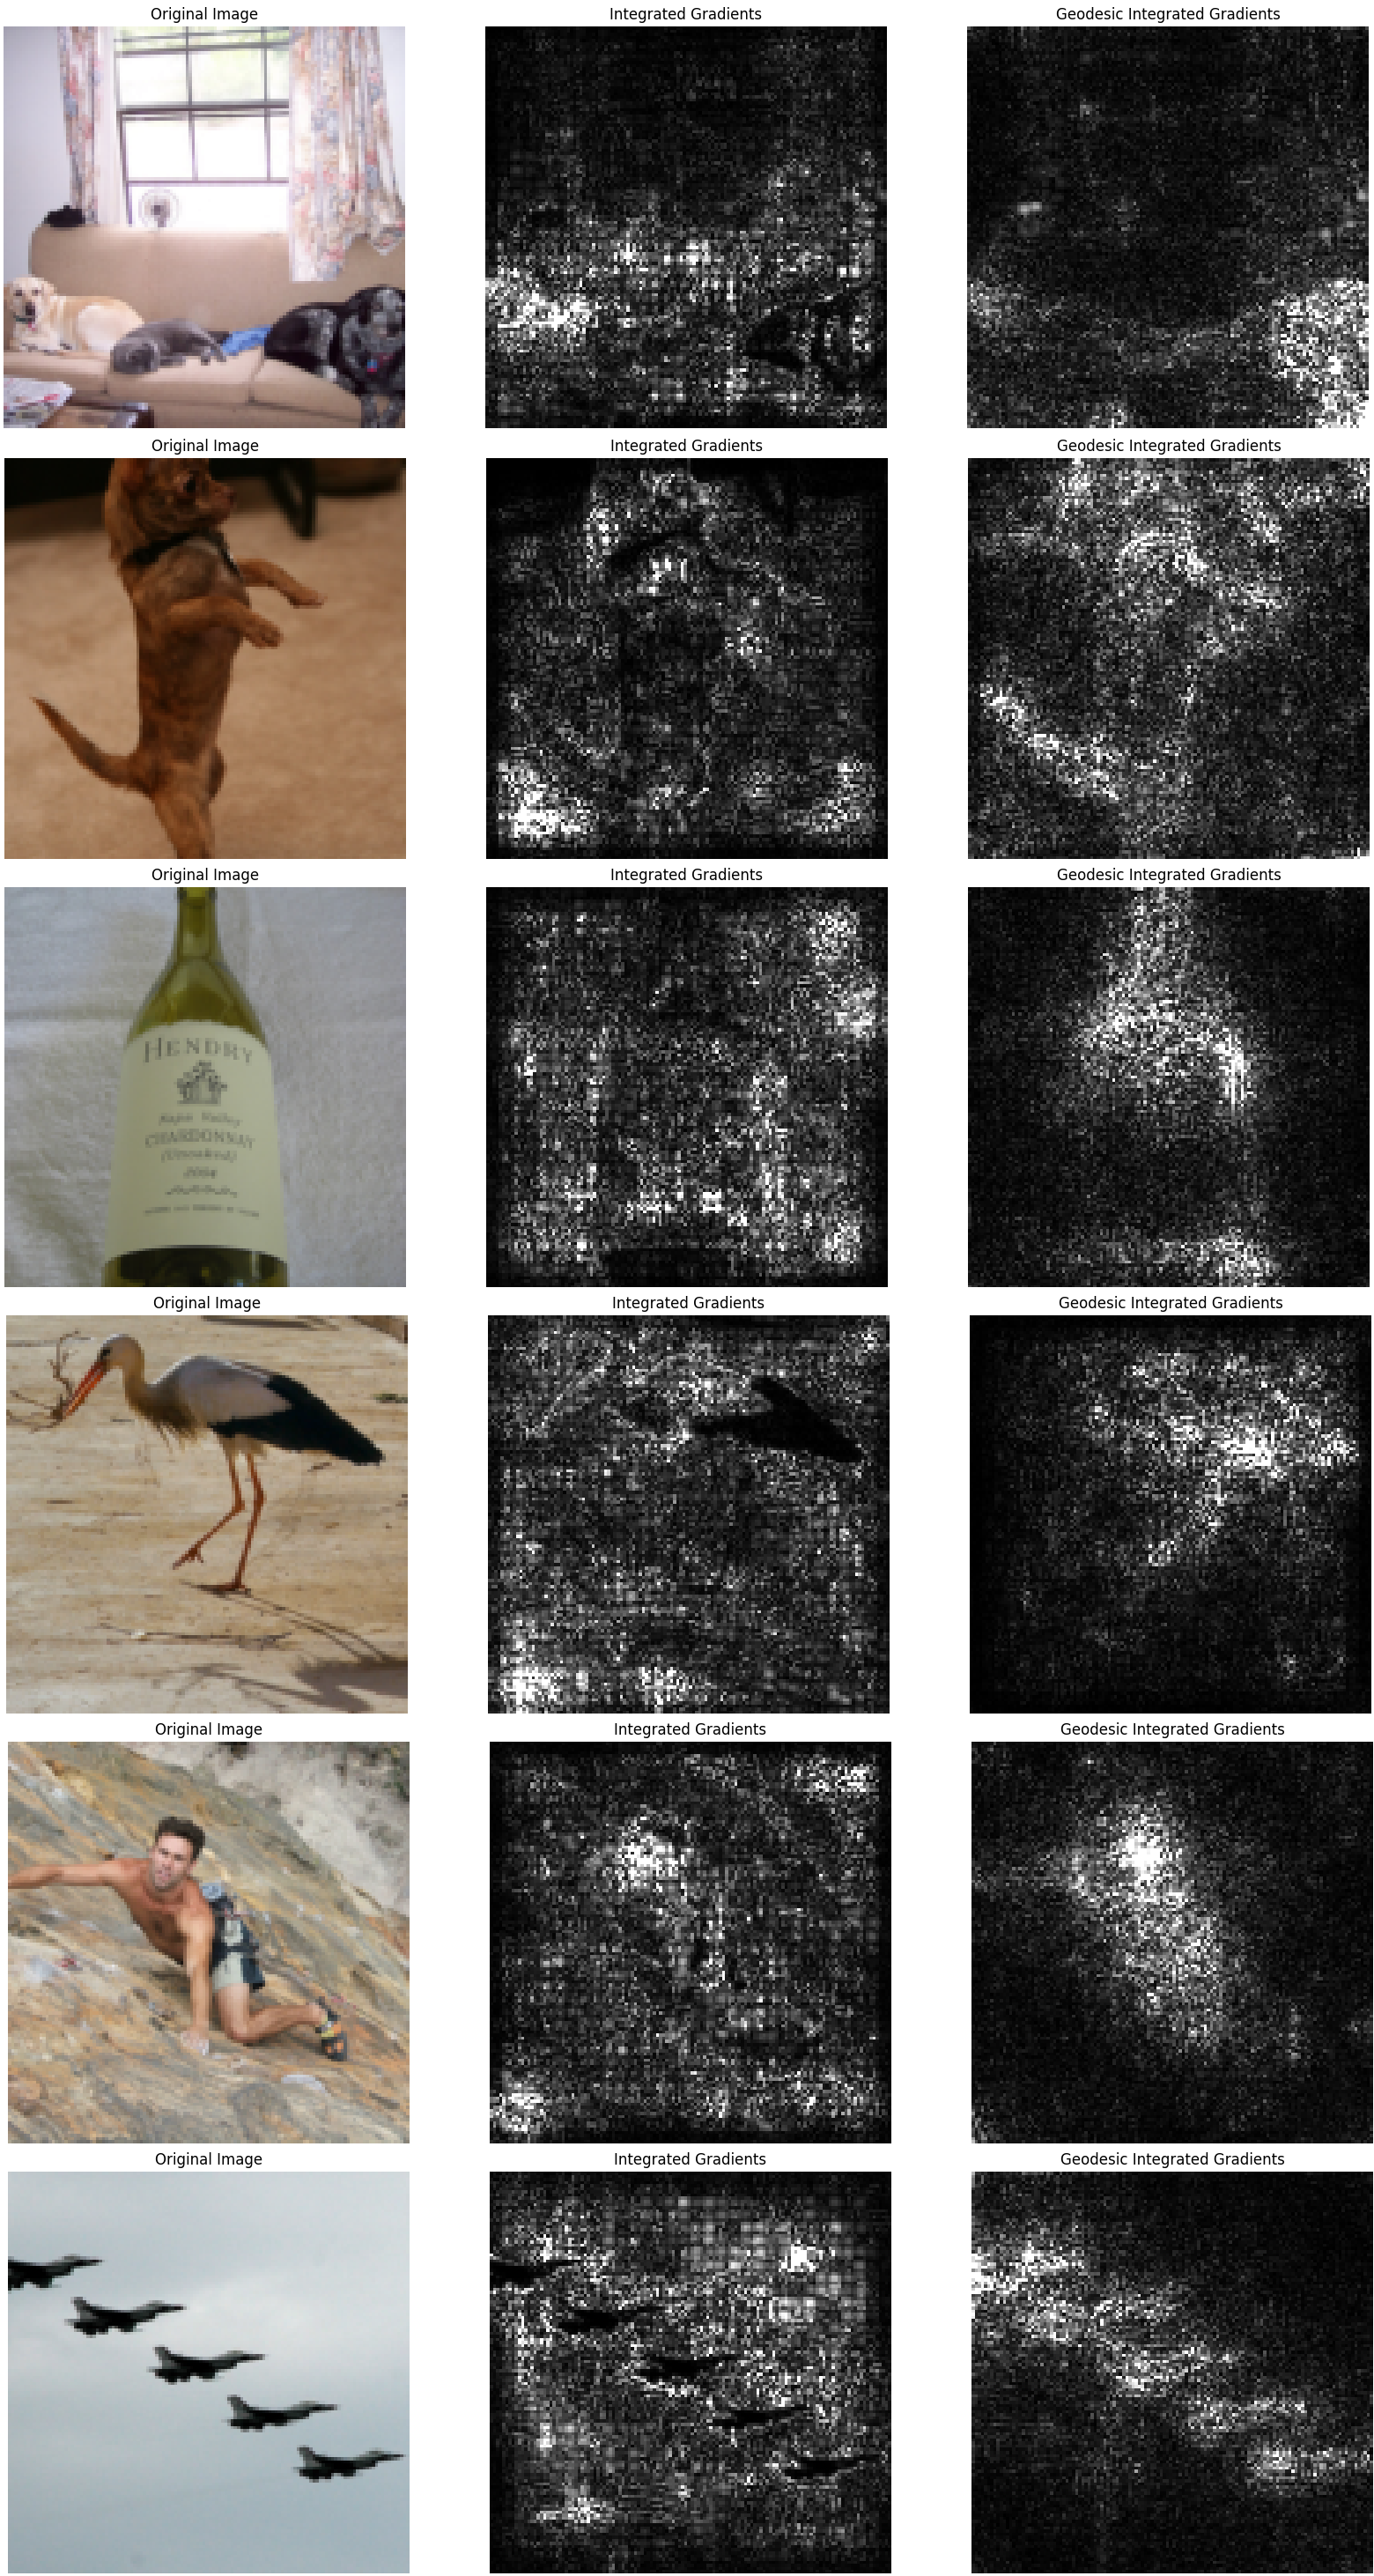
\includegraphics[width=0.52\textwidth]{figures/more_images.png}}
\caption{Heatmaps of Integrated Gradients (middle) and Geodesic IG (right) on 5 randomly chosen images from the test set of Pascal VOC 2012. We can see that Geodesic IG heatmaps are sharper compared with the original IG method.}
\label{fig:more_images}
\end{center}
\vskip -0.2in
\end{figure}

%%%%%%%%%%%%%%%%%%%%%%%%%%%%%%%%%%%%%%%%%%%%%%%%%%%%%%%%%%%%%%%%%%%%%%%%%%%%%%%
%%%%%%%%%%%%%%%%%%%%%%%%%%%%%%%%%%%%%%%%%%%%%%%%%%%%%%%%%%%%%%%%%%%%%%%%%%%%%%%


\end{document}


% This document was modified from the file originally made available by
% Pat Langley and Andrea Danyluk for ICML-2K. This version was created
% by Iain Murray in 2018, and modified by Alexandre Bouchard in
% 2019 and 2021 and by Csaba Szepesvari, Gang Niu and Sivan Sabato in 2022. 
% Previous contributors include Dan Roy, Lise Getoor and Tobias
% Scheffer, which was slightly modified from the 2010 version by
% Thorsten Joachims & Johannes Fuernkranz, slightly modified from the
% 2009 version by Kiri Wagstaff and Sam Roweis's 2008 version, which is
% slightly modified from Prasad Tadepalli's 2007 version which is a
% lightly changed version of the previous year's version by Andrew
% Moore, which was in turn edited from those of Kristian Kersting and
% Codrina Lauth. Alex Smola contributed to the algorithmic style files.
